\documentclass[10pt]{beamer}
\usepackage{graphicx}
\usepackage{adjustbox}
\usepackage{hyperref}
\usepackage{amsmath}
\usepackage{hyperref}
\usepackage{graphicx}
\usepackage{float}
\usepackage{caption}
\usepackage{listings}
\usepackage{xcolor}
\usepackage{multimedia}


% Define colors
\colorlet{punct}{red!60!black}
\definecolor{background}{RGB}{240, 248, 255} % Pale Blue
\definecolor{delim}{RGB}{20,105,176}
\colorlet{numb}{magenta!60!black}

% Define JSON language
\lstdefinelanguage{json}{
    basicstyle=\ttfamily\footnotesize\color{black},
    numbers=left,
    numberstyle=\scriptsize,
    stepnumber=1,
    numbersep=8pt,
    showstringspaces=false,
    breaklines=true,
    frame=lines,
    backgroundcolor=\color{background},
    literate=
     *{0}{{{\color{numb}0}}}{1}
      {1}{{{\color{numb}1}}}{1}
      {2}{{{\color{numb}2}}}{1}
      {3}{{{\color{numb}3}}}{1}
      {4}{{{\color{numb}4}}}{1}
      {5}{{{\color{numb}5}}}{1}
      {6}{{{\color{numb}6}}}{1}
      {7}{{{\color{numb}7}}}{1}
      {8}{{{\color{numb}8}}}{1}
      {9}{{{\color{numb}9}}}{1}
      {:}{{{\color{punct}{:}}}}{1}
      {,}{{{\color{punct}{,}}}}{1}
      {\{}{{{\color{delim}{\{}}}}{1}
      {\}}{{{\color{delim}{\}}}}}{1}
      {[}{{{\color{delim}{[}}}}{1}
      {]}{{{\color{delim}{]}}}}{1},
}


\lstset{frame=single, showstringspaces=false, columns=fixed, basicstyle={\ttfamily}, commentstyle={\it}, numbers=left, tabsize=4}

\definecolor{codebackground}{RGB}{240, 248, 255} % Pale Blue
\definecolor{codecomment}{RGB}{106,153,85}
\definecolor{codekeyword}{RGB}{30,30,255}
\definecolor{codestring}{RGB}{163,21,21}
\definecolor{codenumber}{RGB}{100,100,100}

\lstdefinestyle{modernstyle}{
    backgroundcolor=\color{codebackground},
    commentstyle=\color{codecomment},
    keywordstyle=\color{codekeyword},
    numberstyle=\tiny\color{codenumber},
    stringstyle=\color{codestring},
    basicstyle=\ttfamily\footnotesize\color{black},
    breakatwhitespace=false,
    breaklines=true,
    captionpos=b,
    keepspaces=true,
    numbers=left,
    numbersep=5pt,
    showspaces=false,
    showstringspaces=false,
    showtabs=false,
    tabsize=4
}

\lstset{style=modernstyle}

\usetheme{Copenhagen}
\usecolortheme{default}  % You can choose from various color themes provided by metropolis
% \setbeamertemplate{footline}[frame number]
\setbeamertemplate{navigation symbols}{}

\title[exMA WP1 Vegetation]{
  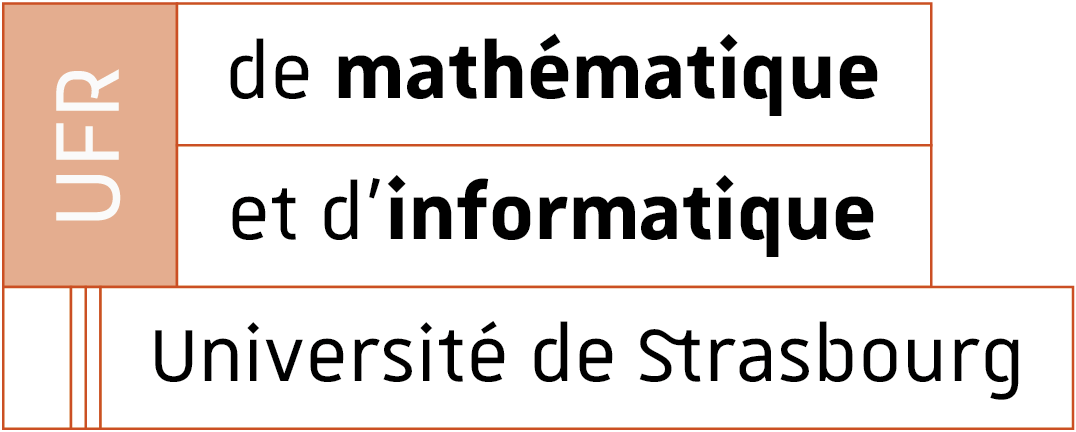
\includegraphics[width=0.8\textwidth]{images/logo_ufr.png}
  Project WP1 - Vegetation}
\author[PA-Giulio]{Giulio CARPI LAPI, Pierre-Antoine SENGER}

\begin{document}

\frame{\titlepage}

\begin{frame}{Context: Hidalgo2}
  \begin{figure}[H]
    \begin{itemize}
      \item Part of the \textbf{HiDALGO2}\cite{hidalgo2} project, focusing on the Urban Building Model (UBM) use case.
      \item Context:
      \begin{itemize}
        \item 75\% of EU building stock is energy inefficient.
        \item Buildings account for 40\% of EU energy consumption.
        \item Buildings generate 36\% of EU greenhouse gas emissions.
      \end{itemize}
      \item Importance:
      \begin{itemize}
        \item Enhancing building energy efficiency aligns with European Green Deal goals.
        \item Improving thermal comfort and air quality affects well-being, productivity, and health.
        \item Climate change increases the urgency for effective building management tools.
      \end{itemize}
    \end{itemize}
    \centering
    \includegraphics[width=0.6\textwidth]{images/hidalgo2.png}
    \captionsetup{font={scriptsize}}
\end{figure}
\end{frame}

\begin{frame}{Context : Impact of vegetation on urban heat}
  \begin{figure}[H]
    \centering
    \begin{minipage}{0.49\textwidth}
        \centering
        \includegraphics[width=\textwidth]{images/TreeShade.png}
        \captionsetup{font={scriptsize}}
        \caption{Tree providing shade to a building \cite{img:TreeShade}.}
    \end{minipage}\hfill
    \begin{minipage}{0.49\textwidth}
        \centering
        \includegraphics[width=\textwidth]{images/heat_street.png}
        \captionsetup{font={scriptsize}}
        \caption{Thermal image of a street depicting heat distribution \cite{img:street_thermography}.}
    \end{minipage}
  \end{figure}
\end{frame}

\begin{frame}{Objectives}
  \begin{figure}[H]
    \centering
    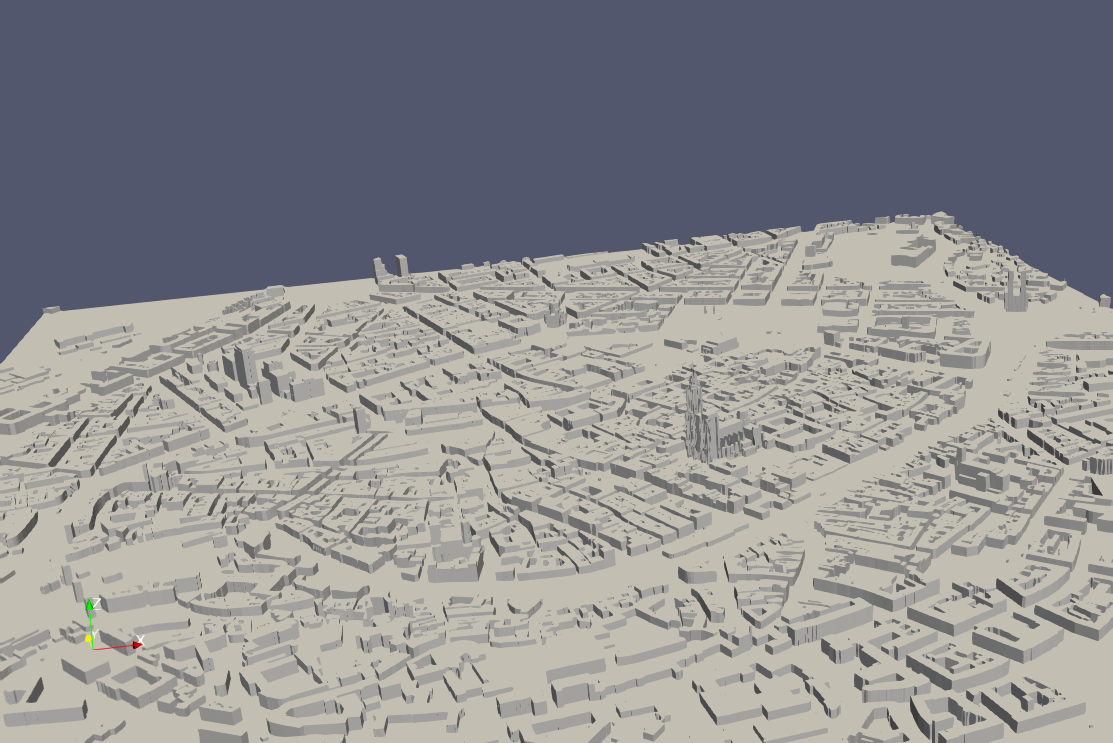
\includegraphics[width=1\textwidth]{images/stras_mesh.png}
    \captionsetup{font={scriptsize}}
    \caption{Strasbourg 3D model.}
  \end{figure}
\end{frame}

\begin{frame}{Manhattan 3D model}
  \begin{figure}[H]
    \centering
    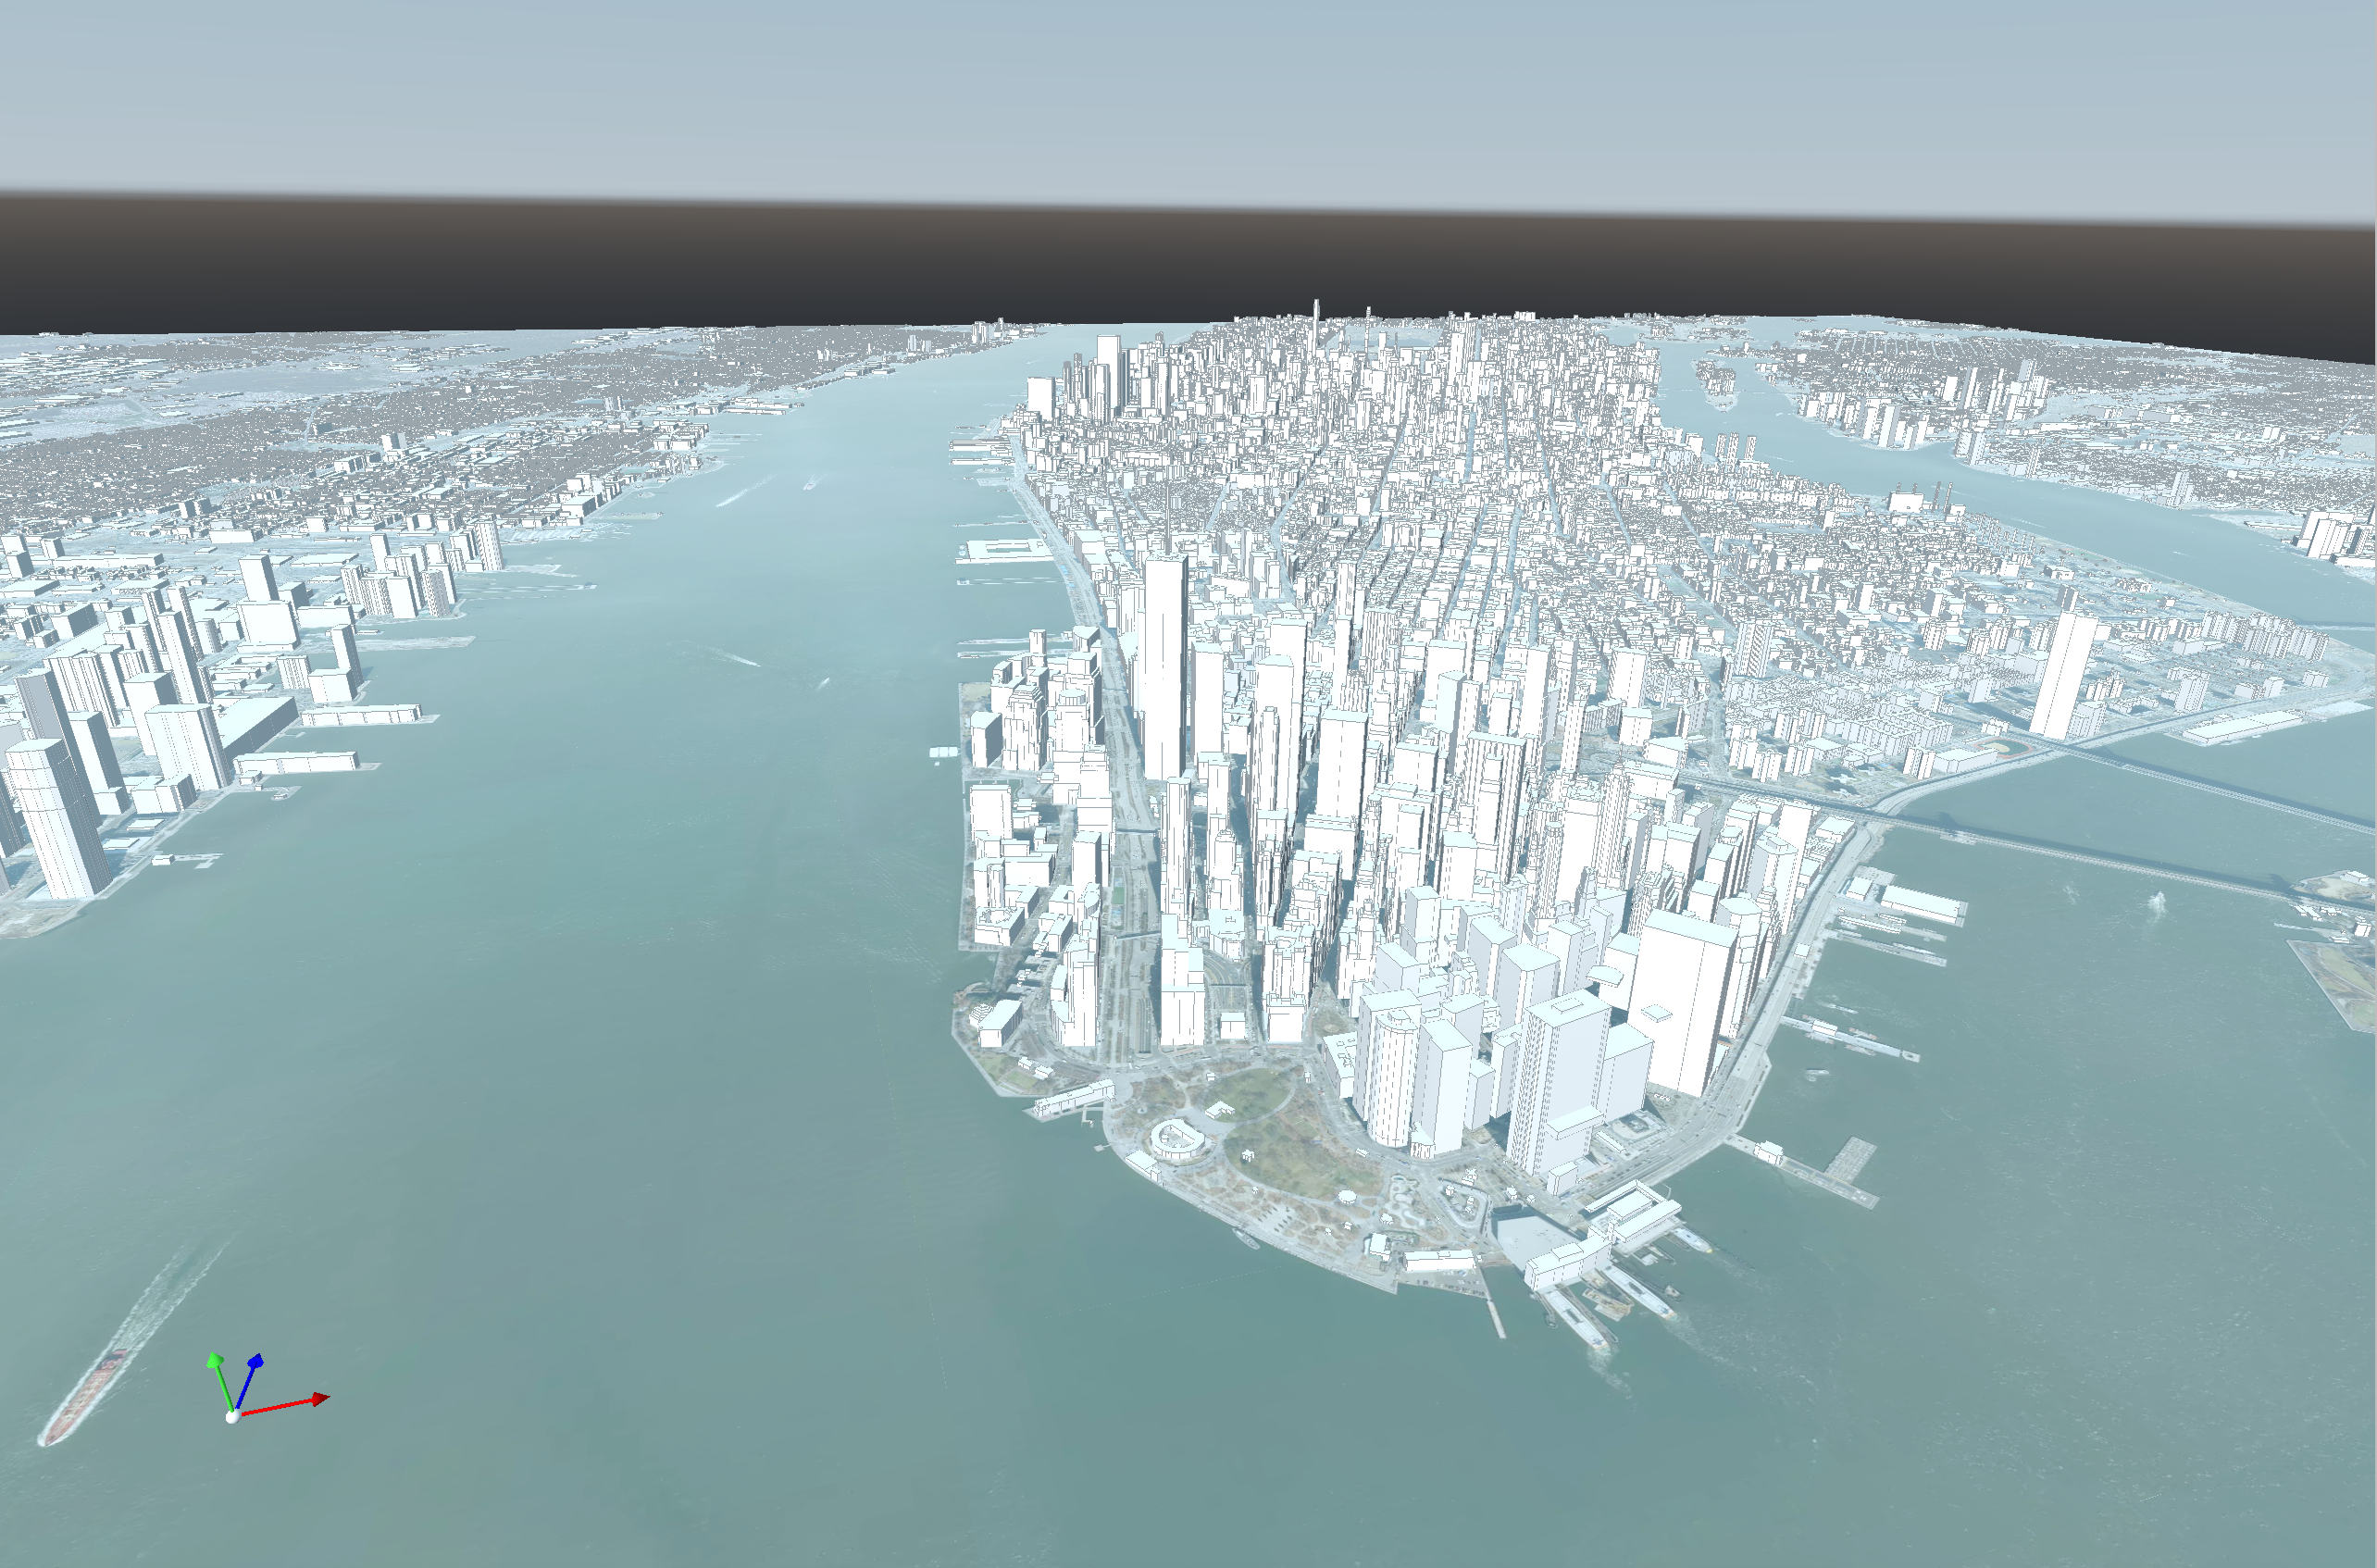
\includegraphics[width=1\textwidth]{images/manhattan_mesh.png}
    \captionsetup{font={scriptsize}}
    \caption{Manhattan 3D model.}
  \end{figure}
\end{frame}

\begin{frame}{Objectives}
  Main objectives: 
  \begin{itemize}
  \item run \textbf{sun masks} using the \textbf{Feel++} library.
  \end{itemize}
  \vspace{0.5cm}

\begin{itemize}
    \item Extracting tree data from \texttt{OpenStreetMap}
    \item Generating 3D tree models.
    \item Integrating tree models into terrain meshes.
    \item Simulating how trees influence energy consumption and microclimates.
\end{itemize}
\end{frame}

\begin{frame}{Starting point}
  We have :
  \begin{itemize}
    \item Scientific articles \cite{Verdie14} \cite{Verdie15} \cite{Stava14} ...
    \item CGAL\cite{cgal} C++ library to mesh trees \includegraphics[width=0.2\textwidth]{images/cgal_logo.png}
    \item Feel++\cite{feel++} C++ library to run simulations 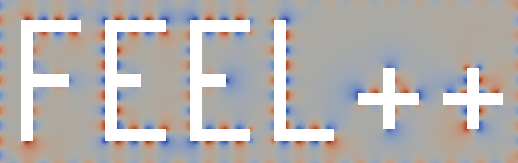
\includegraphics[width=0.2\textwidth]{images/feelpp.png}
    \item A 3D model of Strasbourg
  \end{itemize}
\end{frame}

\begin{frame}{Methodology: data acquisition}
  Use \textbf{OpenStreetMap} API to get the data about the trees in Strasbourg.

  \begin{figure}[H]
    \centering
    \begin{minipage}{0.49\textwidth}
        \centering
        
\includegraphics[width=\textwidth]{images/osm_logo.png}
        \captionsetup{font={scriptsize}}
        \caption{Overpass logo.}
    \end{minipage}\hfill
    \begin{minipage}{0.49\textwidth}
        \centering
        \includegraphics[width=\textwidth]{images/OvAPI_logo.png}
        \captionsetup{font={scriptsize}}
        \caption{Overpass API logo.}
    \end{minipage}
  \end{figure}
\end{frame}

\begin{frame}{Data acquisition: how API works}
  \begin{figure}[H]
    \centering
    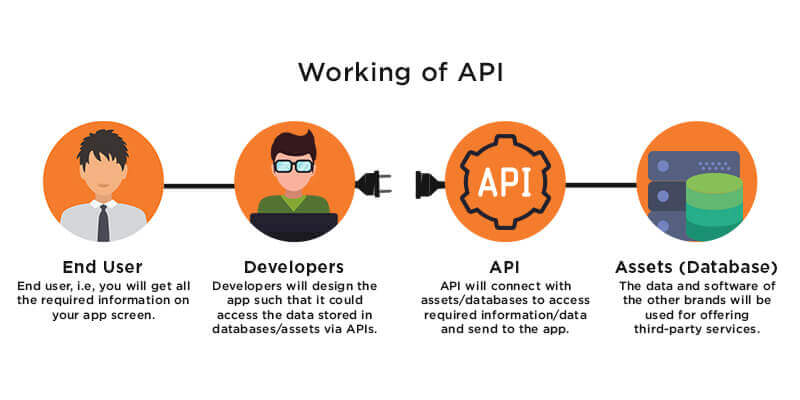
\includegraphics[width=1\textwidth]{images/how-api-works.jpg}
    \captionsetup{font={scriptsize}}
    \caption{Example of query to get trees in Strasbourg.}
  \end{figure}
\end{frame}

\begin{frame}{Data acquisition: Overpass turbo}
\href{https://overpass-turbo.eu/}{Overpass turbo}
 is a web-based data filtering tool for OpenStreetMap. 
It runs queries on the Overpass API.

  \begin{figure}[H]
    \centering
    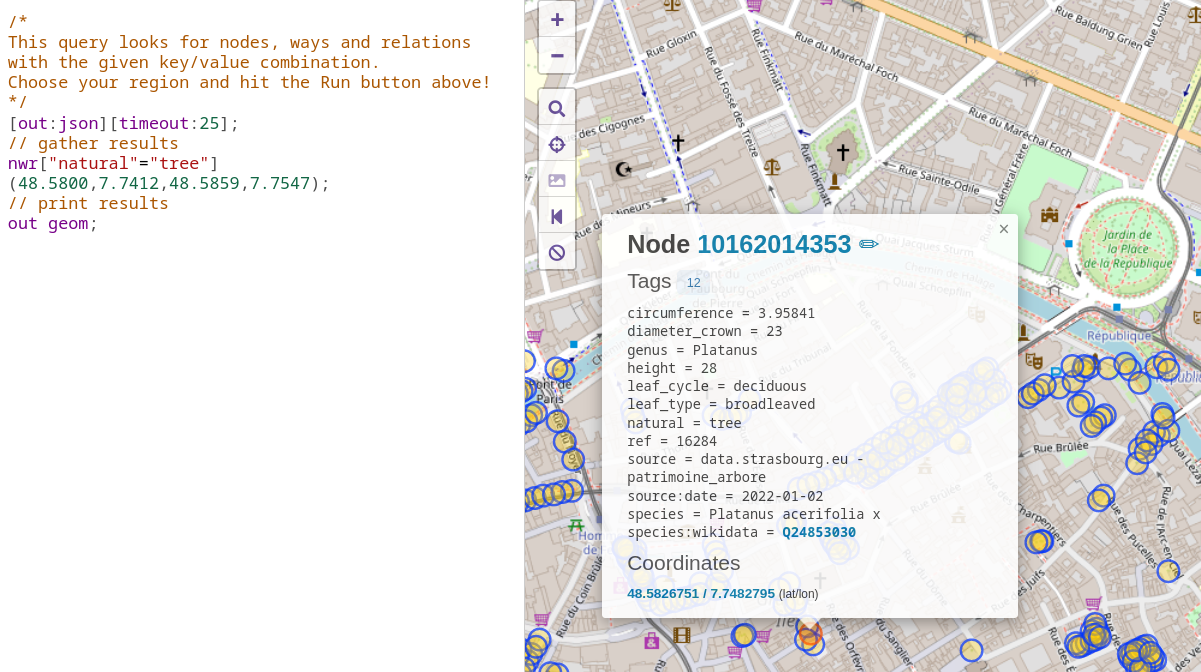
\includegraphics[width=1\textwidth]{images/overpass_turbo.png}
    \captionsetup{font={scriptsize}}
    \caption{Example of query to get trees in Strasbourg using Overpass turbo.}
  \end{figure}
\end{frame}

\begin{frame}[fragile]{Data acquisition: Curl}
  
\includegraphics[width=0.2\textwidth]{images/Curl-logo.svg.png}is a command-line tool to transfer data with URL syntax.
  We're using a configuration file \textit{config.json} to specify the query parameters.
  Here is an example of a configuration file:
\begin{lstlisting}[language=json]
{
  "bbox": "48.5866,7.7522,48.5876,7.7557",
  "origin": "48.583055227464364, 7.748664426560083",
  "LOD": 0,
  "default_height_range": "3, 40",
  "default_genus": "Platanus",
  "input_building_mesh": "mesh_lod1.stl",
  "output_name": "republique"
}
\end{lstlisting}
\end{frame}

\begin{frame}[fragile]{Data acquisition: Curl - Query result} 
  The result of the query is a JSON file \textit{query\_result.json} containing the data about the trees.
Here is the beginning of the file from the previous query:

\begin{lstlisting}[language=json]
{
  "version": 0.6,
  "generator": "Overpass API 0.7.62.1 084b4234",
  "osm3s": {
    "timestamp_osm_base": "2024-05-26T13:31:45Z",
    "copyright": "The data included in this document is from www.openstreetmap.org. The data is made available under ODbL."
  },
  "elements": [
\end{lstlisting}
\end{frame}

\begin{frame}[fragile]{Data acquisition: Curl - Query result}
 The elements are the trees:

\begin{lstlisting}[language=json]
{
  "type": "node",
  "id": 10161978687,
  "lat": 48.5871937,
  "lon": 7.7531245,
  "tags": {
    "circumference": "0.62832",
    "diameter_crown": "5",
    "genus": "Tilia",
    "height": "9",
    "natural": "tree",
    "ref": "27490",
    "source": "data.strasbourg.eu - patrimoine_arbore",
    "source:date": "2022-01-02",
    "species": "Tilia euchlora x"
  }
}, ...
\end{lstlisting}
\end{frame}

\begin{frame}[fragile]{Data acquisition: Curl - Query result}
  A tree with less information:

\begin{lstlisting}[language=json]
{
    "type": "node",
    "id": 4439566691,
    "lat": 48.5839128,
    "lon": 7.7487125,
    "tags": {
      "natural": "tree"
    }
}
\end{lstlisting}
\vfill
How to deal with this case ?
\end{frame}

\begin{frame}{Tree modeling: base tree}
Making all tree model from scratch $\Longrightarrow$ too long. \\
Instead, we're going to start from tree models on \href{https://app.sketchup.com/app}{Sketchup}.

\begin{figure}[H]
    \centering
        \centering
        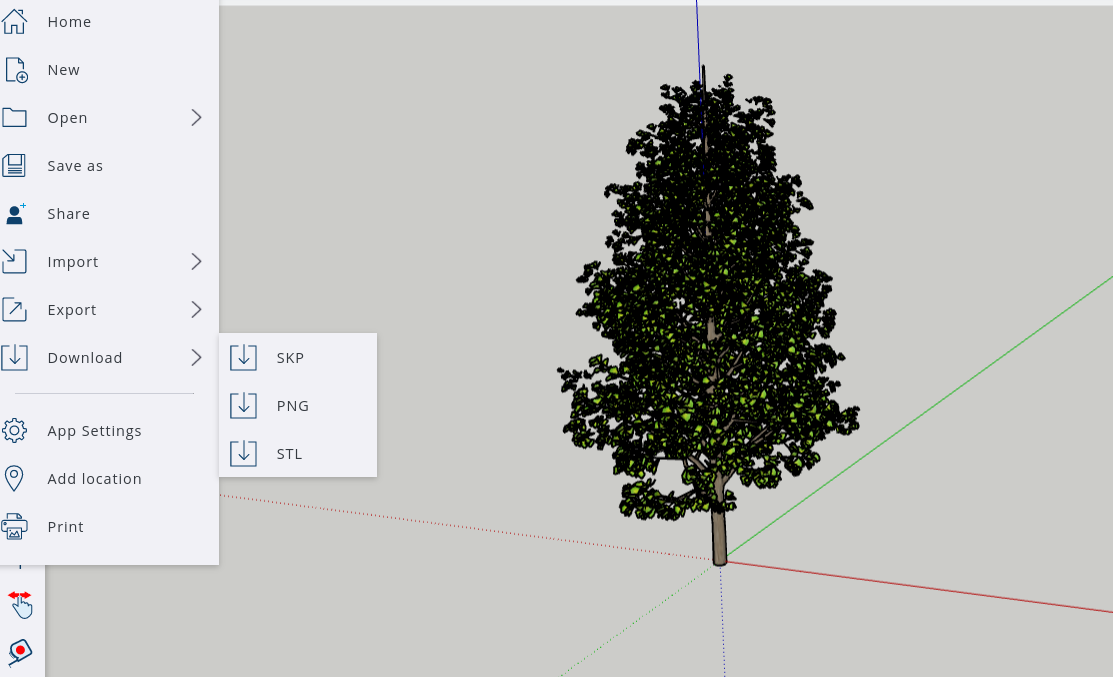
\includegraphics[width=0.8\textwidth]{images/ginkgo_sketchup.png}
        \captionsetup{font={scriptsize}}
        \caption{The mesh of a Ginkgo tree available on Sketchup 3D Warehouse}
\end{figure}
\end{frame}

% \begin{frame}[fragile]{Tree modeling: STL format}

% The \textbf{STL} format\cite{stl_format} is a widely used format for 3D printing and computer-aided design (CAD)
% software. It represents 3D models as a collection of triangular facets, making it
% suitable for our geometric modeling purposes.
% The \texttt{ASCII} versions is defined as :
% \begin{lstlisting}
% solid name
% facet normal ni nj nk
%     outer loop
%         vertex v1x v1y v1z
%         vertex v2x v2y v2z
%         vertex v3x v3y v3z
%     endloop
% endfacet
% ....
% endsolid name
% \end{lstlisting}
% But for efficiency we will use the \texttt{stl} format in its \textbf{binary form}.
% \end{frame}

\begin{frame}{Tree modeling: Alpha Wrapping}
  To provide different LODs we will wrap then using the CGAL 3D 
  Alpha Wrapping\cite{cgal_alpha_wrapper}.

  \begin{figure}[H]
    \centering
        \centering
        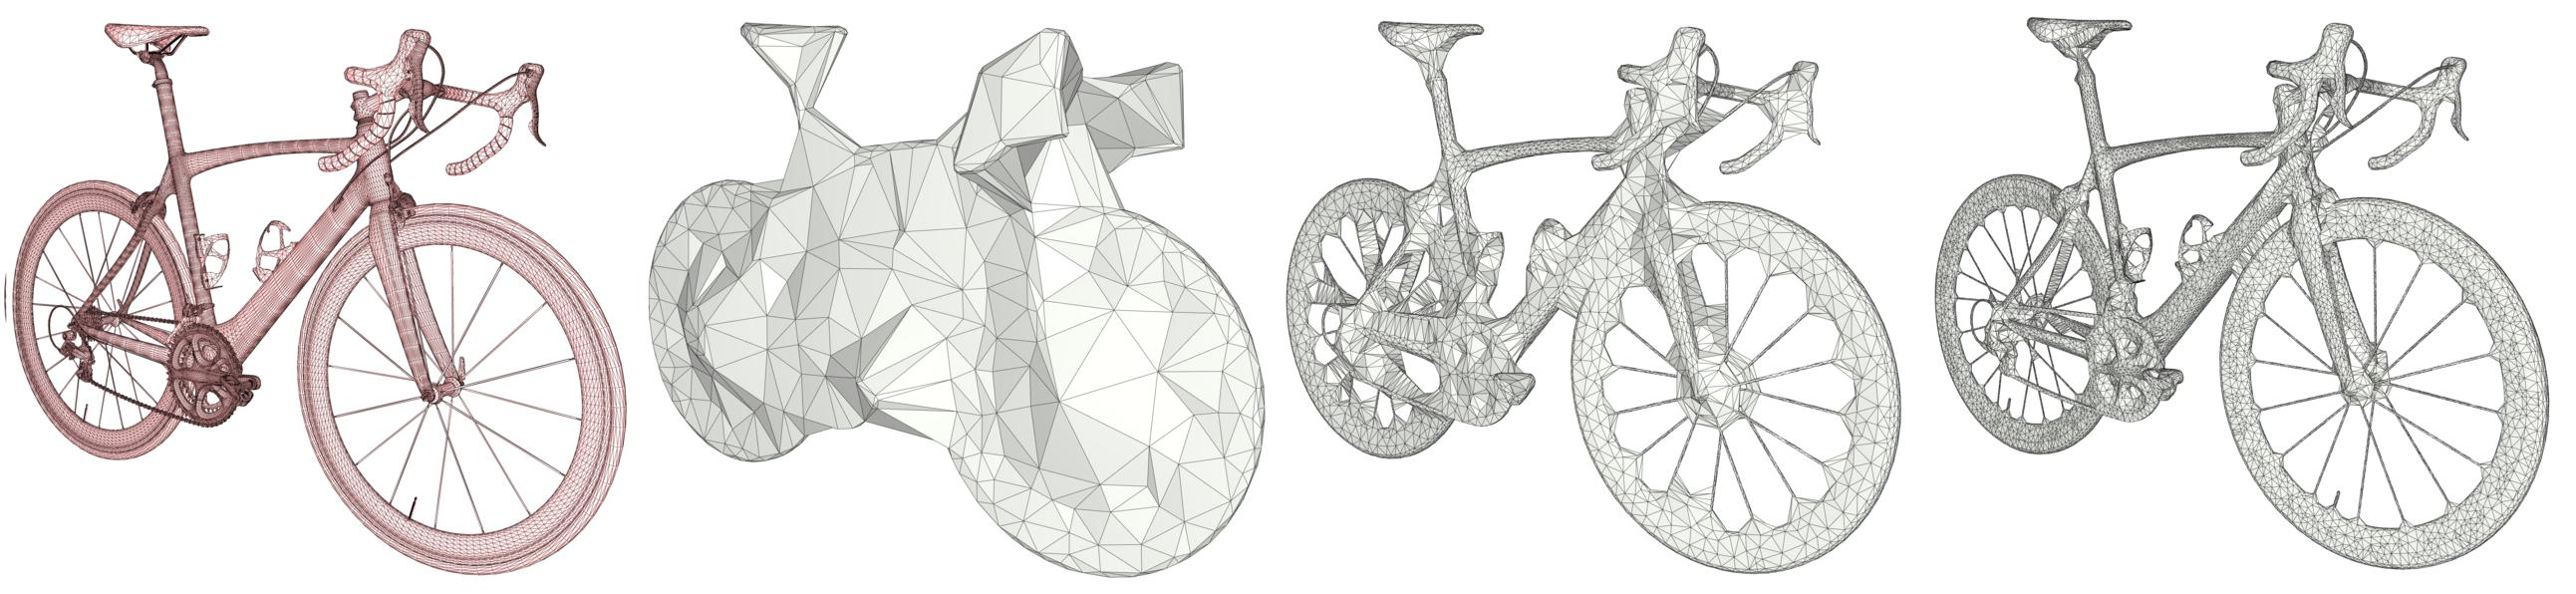
\includegraphics[width=\textwidth]{images/aw3_bike_lod.jpg}
        \captionsetup{font={scriptsize}}
        \caption{Different LOD of the Alpha Wrapping of a bike}
\end{figure}
\end{frame}

\begin{frame}{Reminder: Delaunay triangulation}
  \begin{figure}[H]
    \centering
    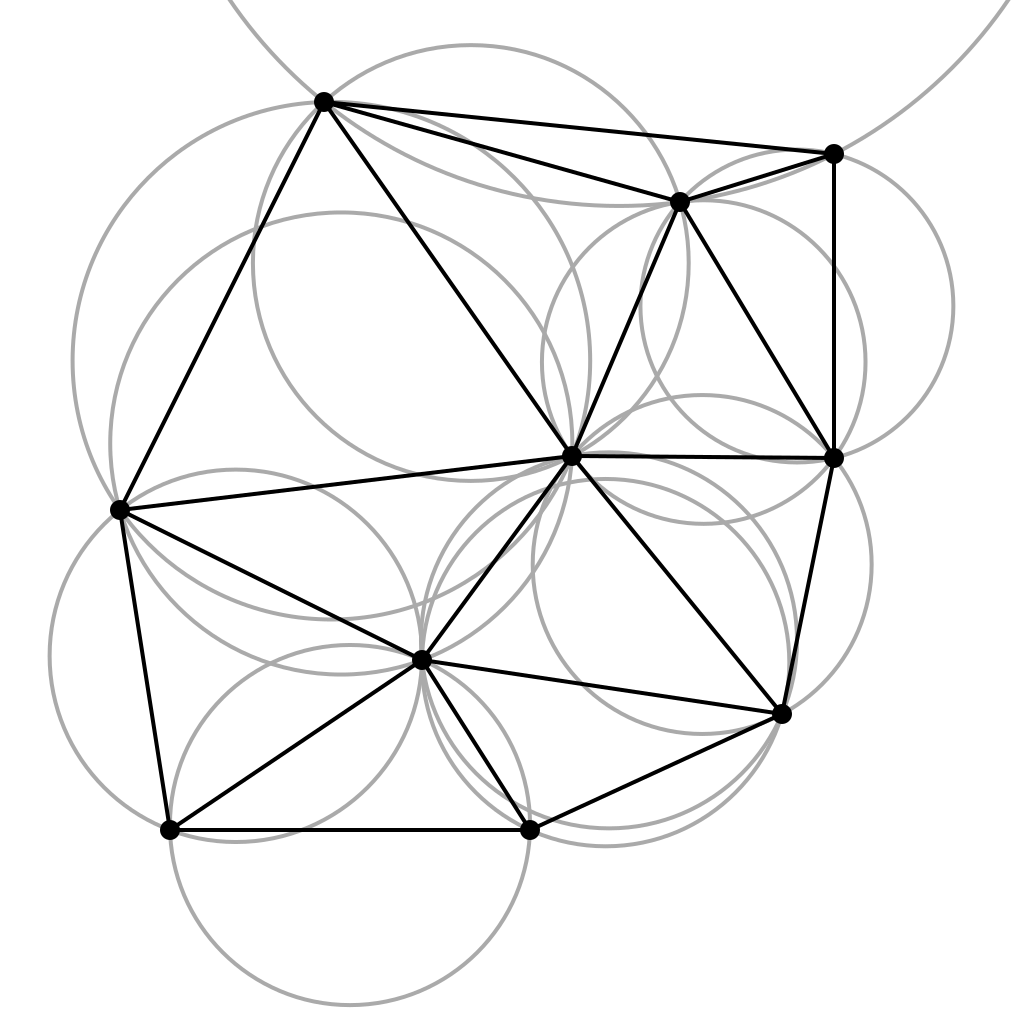
\includegraphics[width=0.6\textwidth]{images/Delaunay_circumcircles_vectorial.svg.png}
    \captionsetup{font={scriptsize}}
    \caption{Delaunay triangulation.
    The circumcircle of each triangle contains no other point.}
\end{figure}
\end{frame}

\begin{frame}{Delaunay and Voronoi}

  \begin{figure}[H]
    \centering
    \begin{minipage}{0.49\textwidth}
        \centering
        \includegraphics[width=\textwidth]{images/Delaunay_circumcircles_centers.svg.png}
        \captionsetup{font={scriptsize}}
        \caption{Delaunay triangulation with the centers of the circumcircles\cite{delaunay-wiki}.}
    \end{minipage}\hfill
    \begin{minipage}{0.49\textwidth}
        \centering
        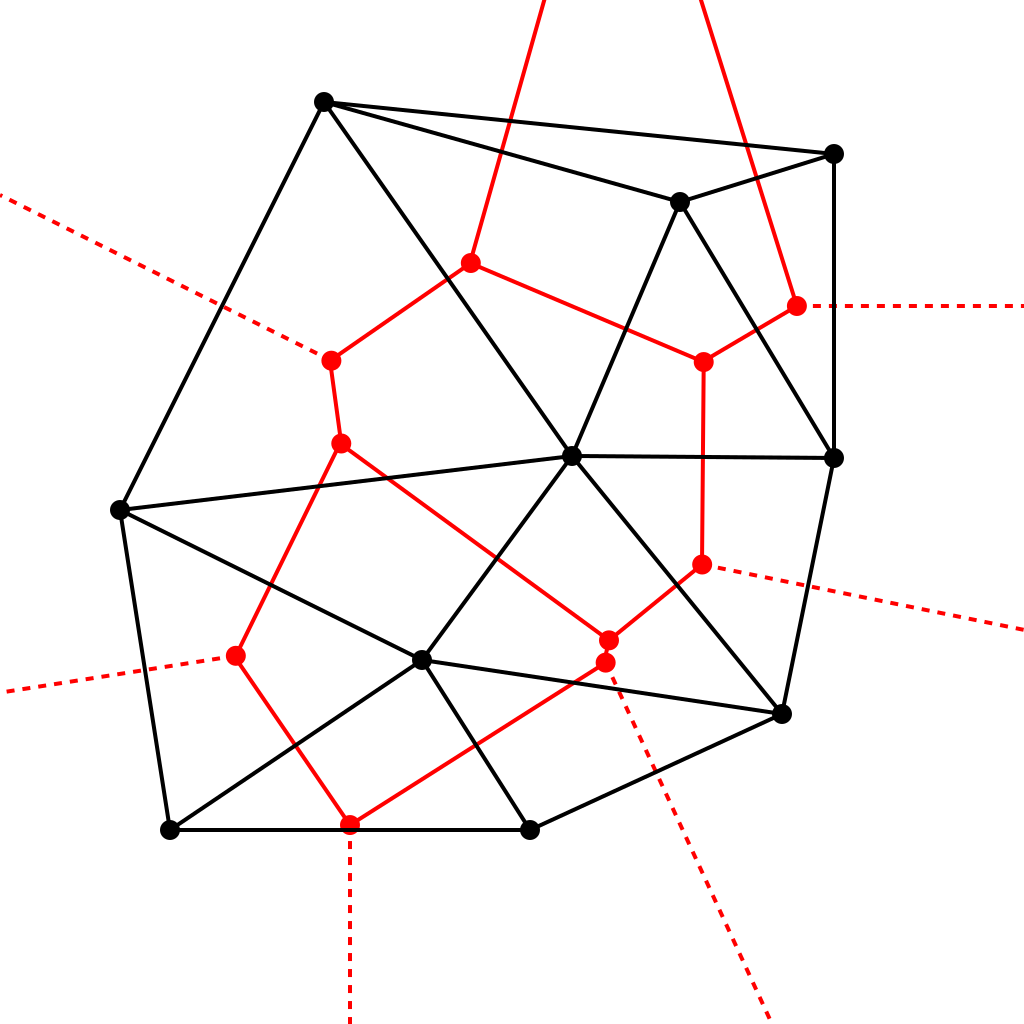
\includegraphics[width=\textwidth]{images/Delaunay_Voronoi.svg.png}
        \captionsetup{font={scriptsize}}
        \caption{The dual of the Delaunay triangulation, the Voronoi diagram\cite{delaunay-wiki}.}
    \end{minipage}
  \end{figure}
\end{frame}



\begin{frame}{Alpha Wrapping}
  \begin{figure}[H]
    \hspace*{-1cm}
    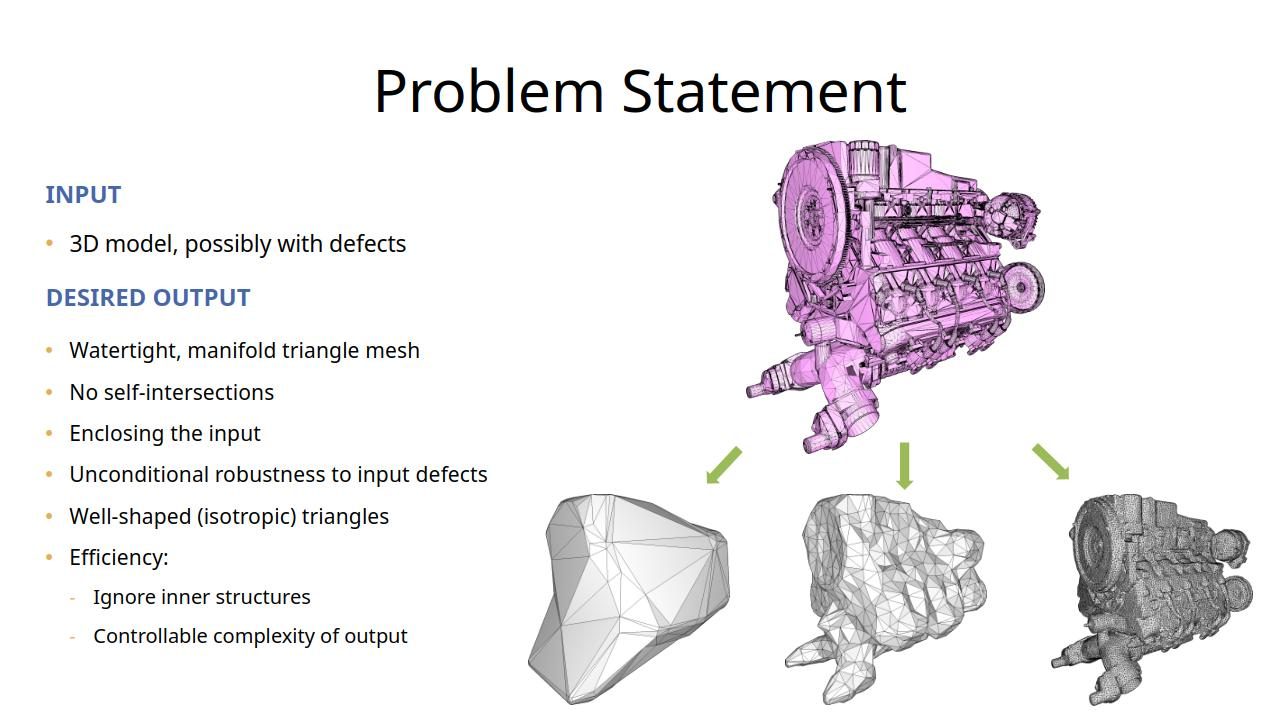
\includegraphics[width=1.2\textwidth]{images/alpha-wrapping.jpg}
  \end{figure}
\end{frame}

\begin{frame}{Alpha Wrapping}
  \begin{figure}[H]
    \centering
    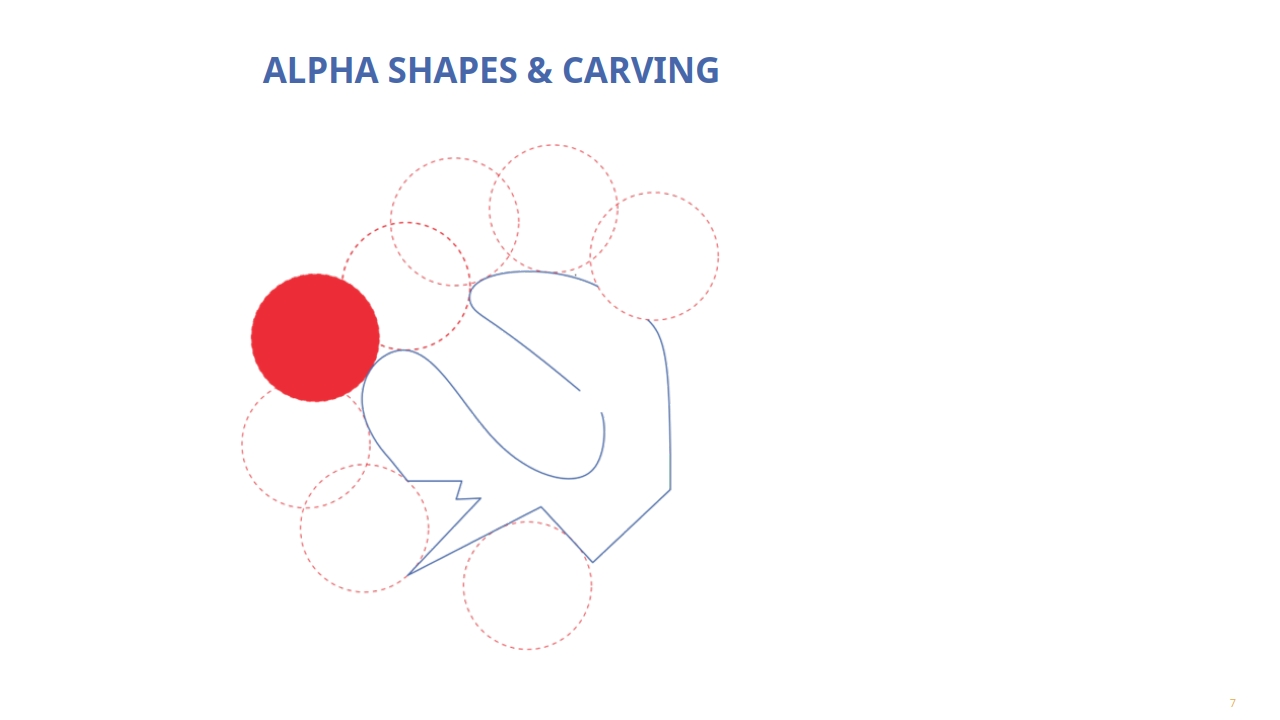
\includegraphics[width=1.1\textwidth]{images/alpha-wrapping1.jpg}
    \captionsetup{font={scriptsize}}
    \caption{Alpha Wrapping in 2D.}
\end{figure}
\end{frame}

\begin{frame}{Alpha Wrapping}
  \begin{figure}[H]
    \centering
    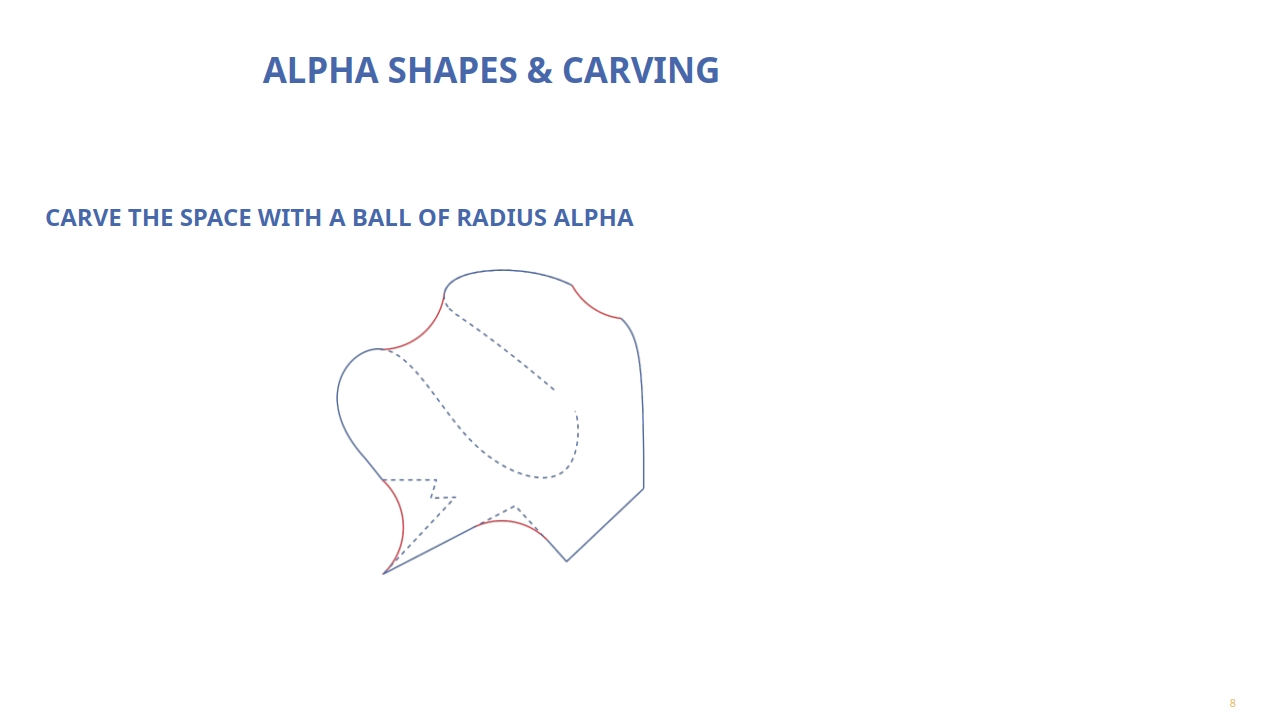
\includegraphics[width=1.1\textwidth]{images/alpha-wrapping2.jpg}
    \captionsetup{font={scriptsize}}
    \caption{Alpha Wrapping in 2D result.}
\end{figure}
\end{frame}

\begin{frame}{Alpha Wrapping}
  \begin{figure}[H]
    \centering
    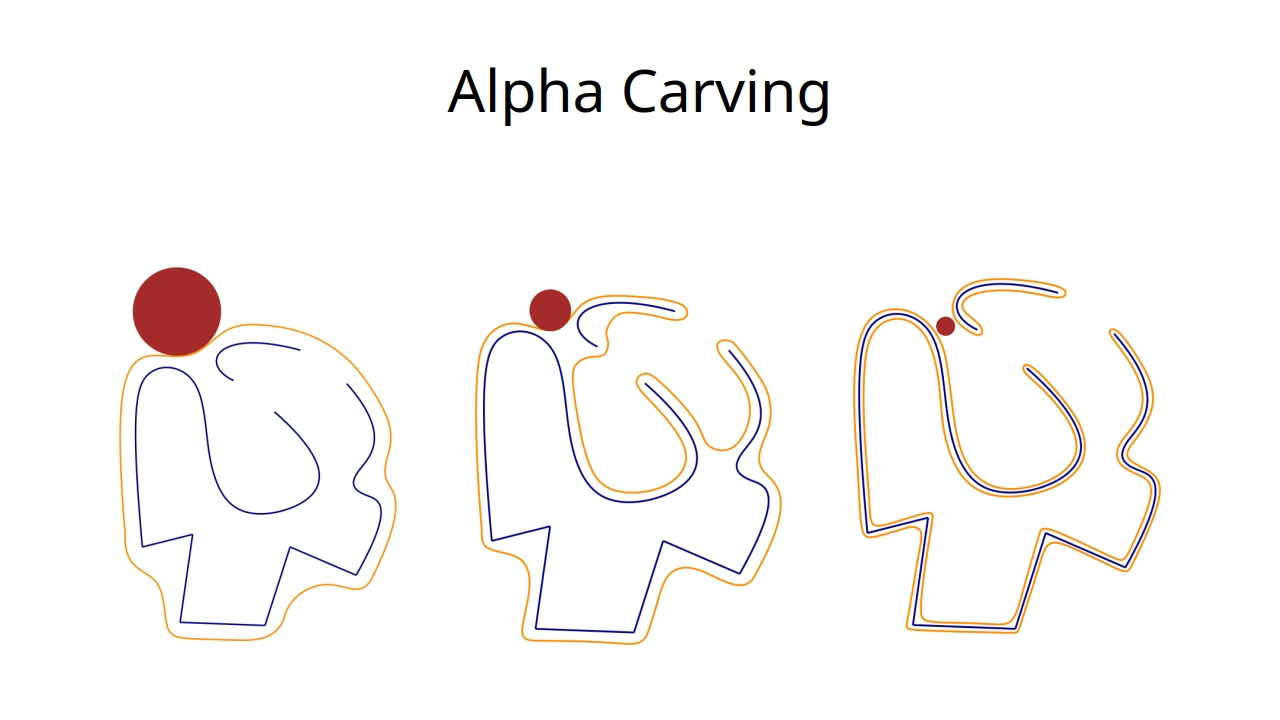
\includegraphics[width=1.1\textwidth]{images/alpha-wrapping3.jpg}
    \captionsetup{font={scriptsize}}
    \caption{Alpha Wrapping in 2D with Offset and different Alpha parameters.}
\end{figure}
\end{frame}

\begin{frame}{Alpha Wrapping}
  \href{https://youtu.be/xIIDolWCrgU}{video link}
  \begin{figure}[H]
    \centering
    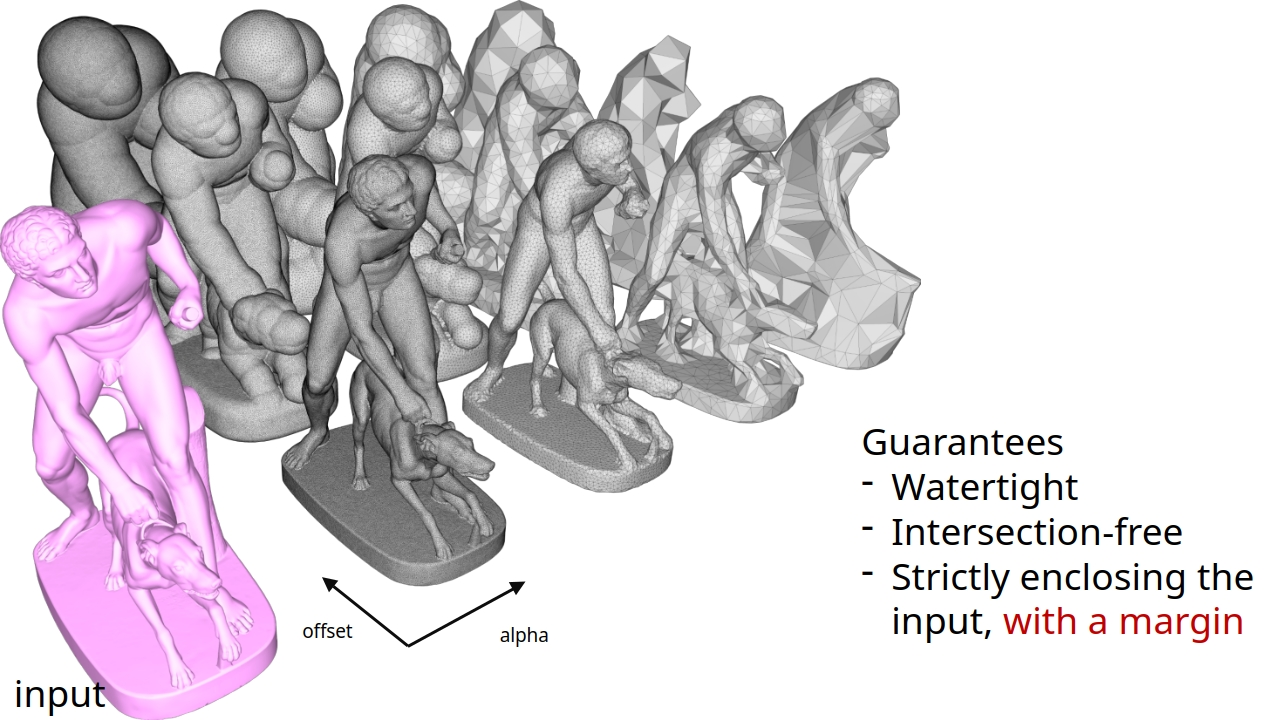
\includegraphics[width=1.1\textwidth]{images/alpha-wrapping4.jpg}
    \captionsetup{font={scriptsize}}
    \caption{Alpha Wrapping Alpha and Offset parameters.}
\end{figure}
\end{frame}

\begin{frame}{Alpha Wrapping animation}
  \href{https://youtu.be/xIIDolWCrgU}{video link}
  \begin{center}
    \movie[width=1\textwidth,height=0.8\textheight,poster,showcontrols]{}{videos/alpha-wrapping-2d.mp4}
\end{center}
\end{frame}

\begin{frame}{Alpha Wrapping tractor}
  \href{https://youtu.be/HG9oHA2NJMM}{video link}
  \begin{center}
    \movie[width=1\textwidth,height=0.8\textheight,poster,showcontrols]{}{videos/tractor.mp4}
\end{center}
\end{frame}

\begin{frame}{Tree modeling: wrapping base tree}
  \begin{figure}[H]
    \centering
    \begin{minipage}{0.49\textwidth}
        \centering
        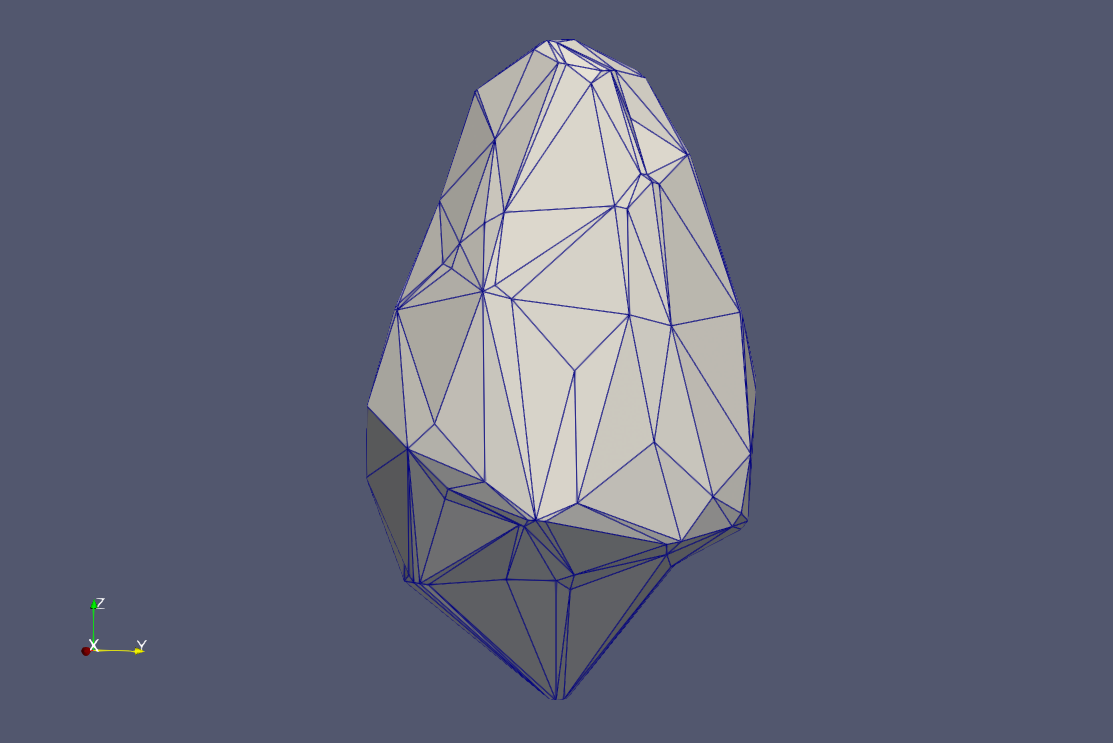
\includegraphics[width=0.8\textwidth]{images/gingko_lod0.png}
        \captionsetup{font={scriptsize}}
        \caption{Ginkgo lod0.}
    \end{minipage}\hfill
    \begin{minipage}{0.49\textwidth}
        \centering
        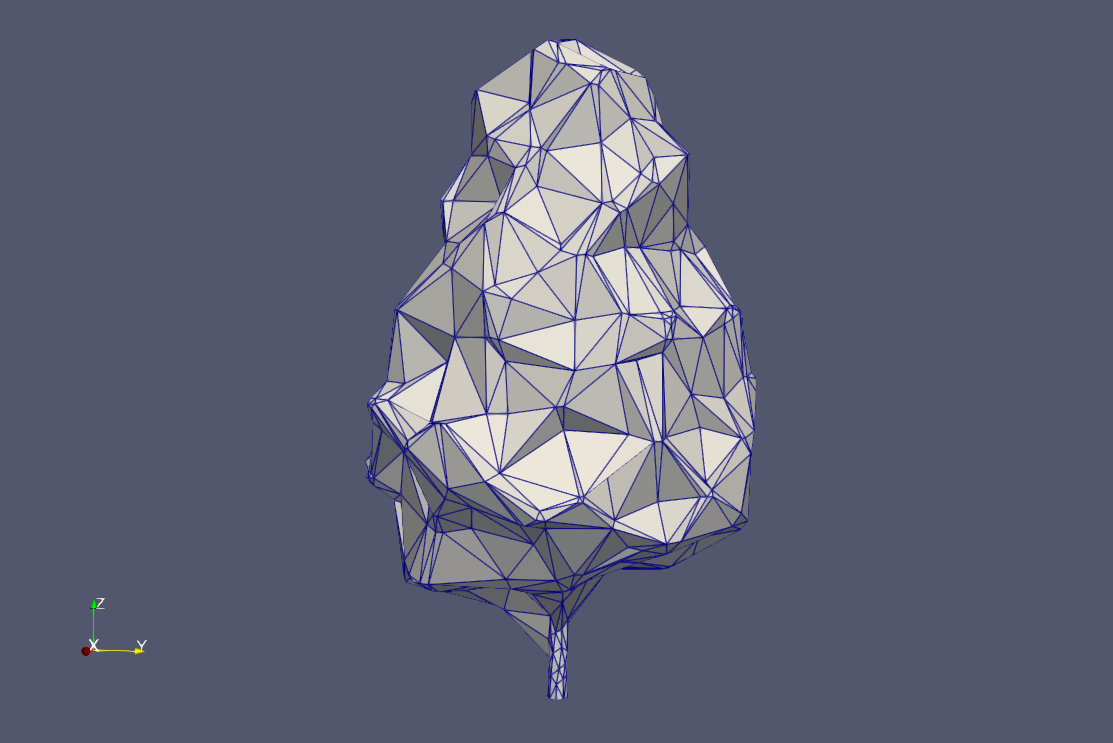
\includegraphics[width=0.8\textwidth]{images/gingko_lod1.png}
        \captionsetup{font={scriptsize}}
        \caption{Ginkgo lod1.}
    \end{minipage}
\end{figure}

\begin{figure}[H]
    \centering
    \begin{minipage}{0.49\textwidth}
        \centering
        \includegraphics[width=0.8\textwidth]{images/gingko_lod2.png}
        \captionsetup{font={scriptsize}}
        \caption{Ginkgo lod2.}
    \end{minipage}\hfill
    \begin{minipage}{0.49\textwidth}
        \centering
        \includegraphics[width=0.8\textwidth]{images/gingko_lod3.png}
        \captionsetup{font={scriptsize}}
        \caption{Ginkgo lod3.}
    \end{minipage}
\end{figure}
\end{frame}

\begin{frame}[fragile]{Tree modeling: tree object}

\begin{lstlisting}[language=C++]
using K = CGAL::Exact_predicates_inexact_constructions_kernel;
using Point_3 = K::Point_3;
using Mesh = CGAL::Surface_mesh<Point_3>;

class Tree {
    private:
    long M_id;
    double M_lat, M_lon, M_x, M_y,
    double M_height, M_circumference, M_diameter_crown
    std::string M_genus, M_species, M_season;
    Mesh M_wrap;

    public:
    void computeXY(double ref_lat, double ref_lon);
    void wrap(int lod);
};

Tree createTreeFromJson(const nlohmann::json &treeJson);
std::ostream &operator<<(std::ostream &os, const Tree &tree);
bool operator<(const Tree &lhs, const Tree &rhs);
\end{lstlisting}
\end{frame}

\begin{frame}{Mercator's projection}
  \begin{figure}[H]
    \centering
    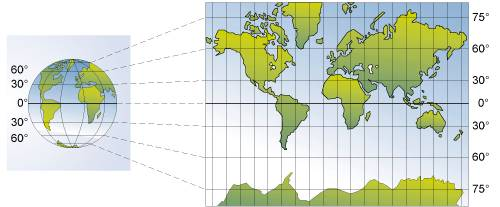
\includegraphics[width=0.8\textwidth]{images/mercator.jpg}
    \captionsetup{font={scriptsize}}
    \caption{Mercator's projection\cite{img:mercator}.}
\end{figure}

\begin{itemize}
  \item Most used projection for representing the Earth's surface on a plane.
  \item Conformal $\Longrightarrow$ preserves angles locally.
  \item Distortion $\Longrightarrow$ relative sizes of countries is not accurate.
\end{itemize}
\end{frame}

\begin{frame}{Mercator's projection}
  \begin{figure}[H]
    \centering
    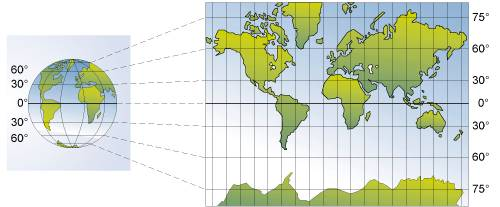
\includegraphics[width=0.8\textwidth]{images/mercator.jpg}
    \captionsetup{font={scriptsize}}
    \caption{Mercator's projection\cite{img:mercator}.}
\end{figure}
Mathematically, the Mercator projection is defined as follows: if a point on 
the sphere has a latitude $\phi$ and longitude $\lambda$ (with $\lambda_{0}$ 
placed at the center of the map), then its projection on the Mercator map will 
have coordinates 
\begin{equation}
  \left\{
  \begin{array}{l}
      x =  \lambda - \lambda_{0} \\
      y =  \ln(\tan(\frac{\pi}{4} + \frac{\phi}{2}))
  \end{array}
  \right.
\end{equation}
\end{frame}

\begin{frame}{Mercator's projection}
  \begin{figure}[H]
    \centering
    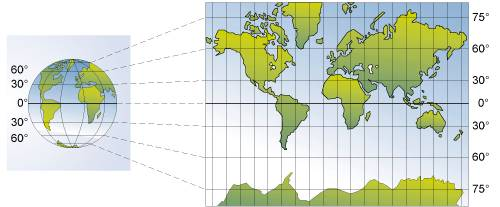
\includegraphics[width=0.8\textwidth]{images/mercator.jpg}
    \captionsetup{font={scriptsize}}
    \caption{Mercator's projection\cite{img:mercator}.}
\end{figure}
But the Earth isn't a perfect sphere...
\end{frame}

\begin{frame}{Mercator's projection}
  \begin{figure}[H]
    \centering
    \begin{minipage}{0.49\textwidth}
        \centering
        \includegraphics[width=0.8\textwidth]{images/WGS84_mean_Earth_radius.svg.png}
        \captionsetup{font={scriptsize}}
        \caption{Earth as an ellipsoid\cite{mercator-wiki}.}
    \end{minipage}\hfill
    \begin{minipage}{0.49\textwidth}
        \centering
        
\includegraphics[width=0.8\textwidth]{images/WGS_84_reference_frame.png}
        \captionsetup{font={scriptsize}}
        \caption{WGS 84 reference frame\cite{mercator-wiki}.}
    \end{minipage}
\end{figure}

We can use the \textit{WGS84toCartesian.hpp}\cite{wgs84_to_cartesian} open source header-only
  library to convert the \textbf{GPS} coordinates so \textbf{Cartesian} coordinates.
\end{frame}

\begin{frame}{Modeling trees in 3D space}
We can use \texttt{CGAL Affine Transformation} \cite{cgal_affine_transformation} 
(complexity in $O(n)$)

\begin{figure}[H]
  \centering
  \begin{minipage}{0.49\textwidth}
      \centering
      \includegraphics[width=1\textwidth]{images/republic_lod3.png}
      \captionsetup{font={scriptsize}}
      \caption{Republic square with LOD 3 trees.}
  \end{minipage}\hfill
  \begin{minipage}{0.49\textwidth}
      \centering
      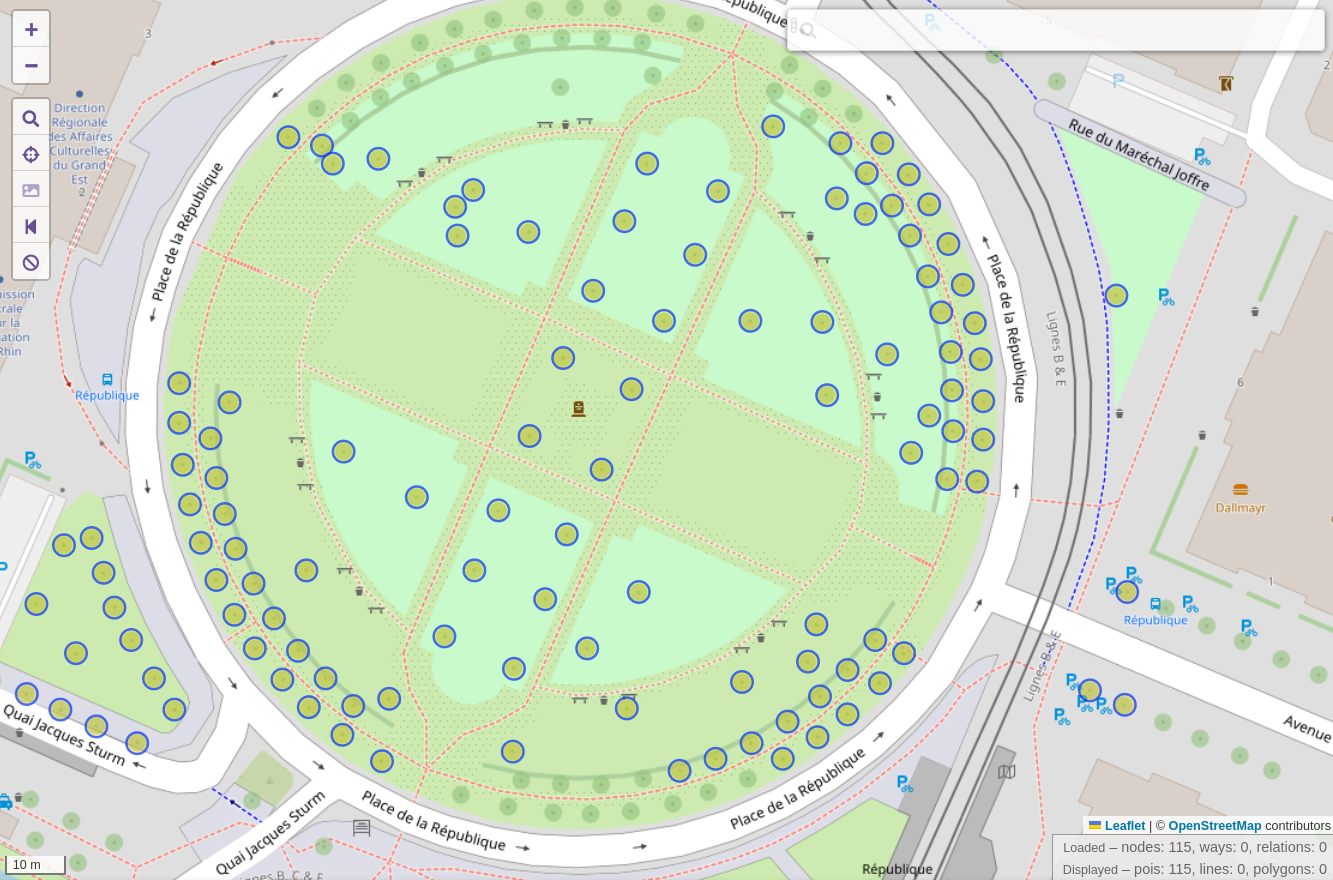
\includegraphics[width=1\textwidth]{images/republic_overpassturbo.png}
      \captionsetup{font={scriptsize}}
      \caption{Republic square trees from Overpass turbo.}
  \end{minipage}
\end{figure}
\end{frame}

\begin{frame}{Modeling trees in 3D space}
  \begin{figure}[H]
    \centering
    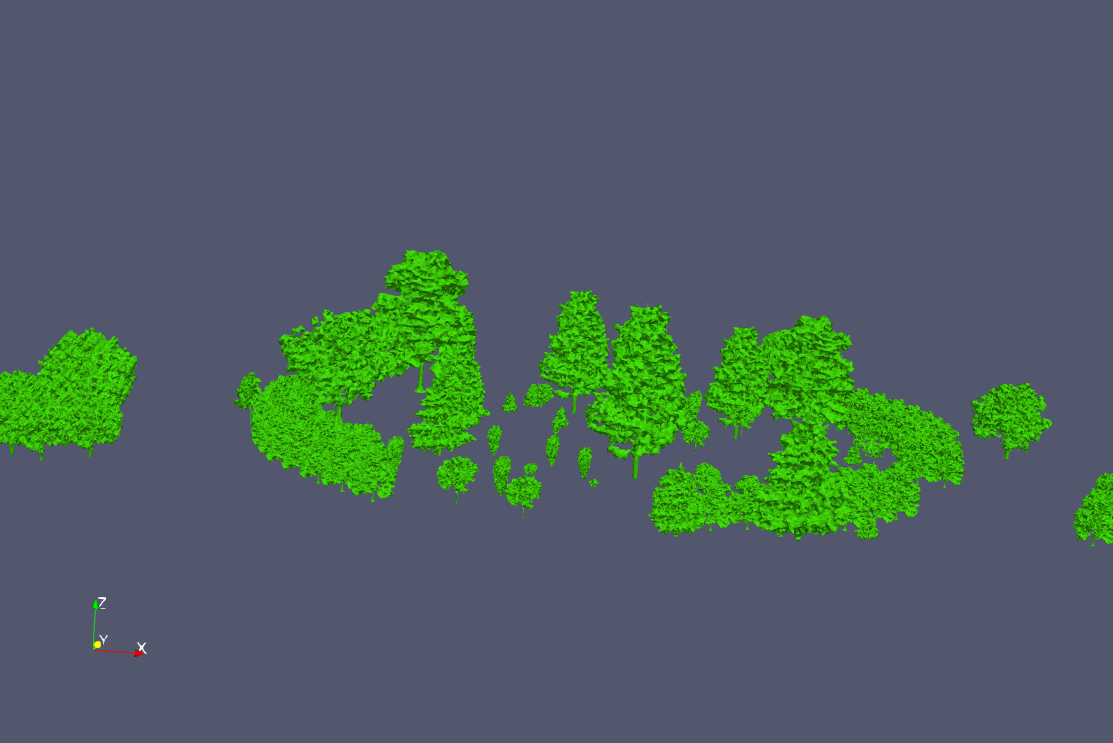
\includegraphics[width=1\textwidth]{images/republic_lod3_side.png}
    \captionsetup{font={scriptsize}}
    \caption{Side view of Republic square with LOD 3 trees.}
\end{figure}
\end{frame}

\begin{frame}{Model integration}
  \begin{figure}[H]
    \centering
    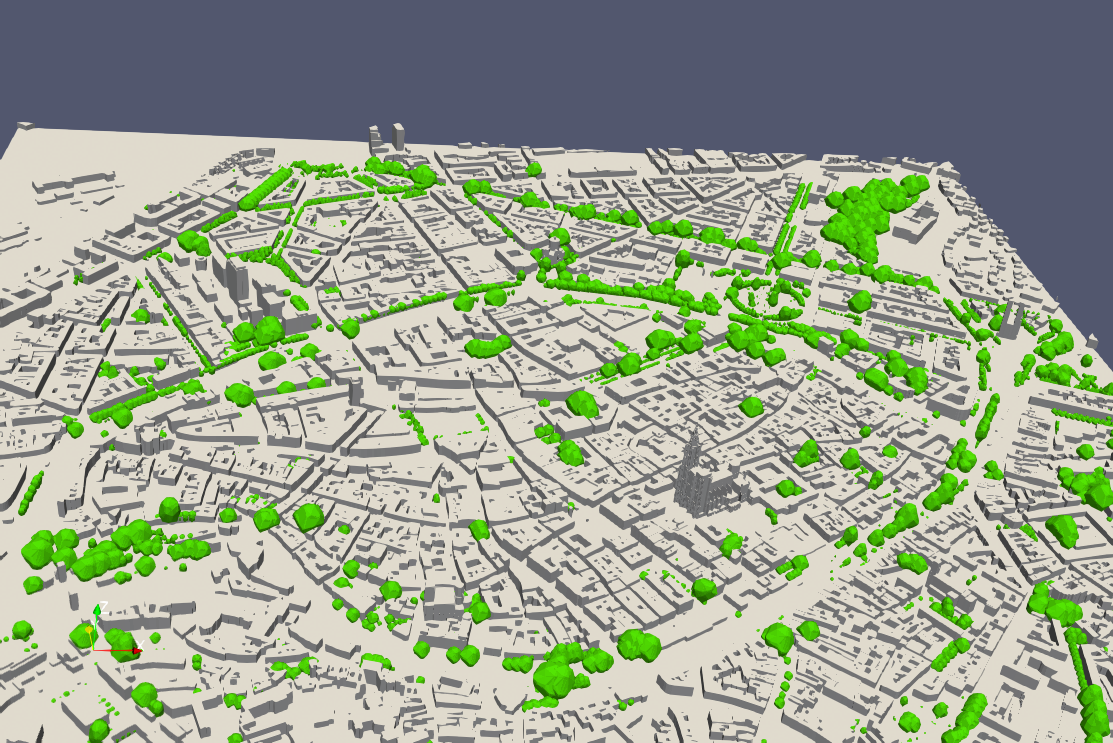
\includegraphics[width=1\textwidth]{images/stras_lod0.png}
    \captionsetup{font={scriptsize}}
    \caption{Strasbourg 3D model with LOD 0 trees.}
\end{figure}
\end{frame}

\begin{frame}{Model integration: prospects}
  Prospects: 
  \begin{itemize}
    \item Use the \texttt{Feel++} library to compute the shading of the trees.
    \item Make the mesh for the Hungarian team $\Longrightarrow$ fluid mechanics simu. 
  \end{itemize}
  \href{https://youtu.be/O6flpW6jR60}{video link}
  \begin{center}
    \movie[width=1\textwidth,height=0.7\textheight,poster,showcontrols]{}{videos/SolarMask.mp4}
\end{center}
\end{frame}

\begin{frame}{Benchmark: bbox 1}
  \begin{figure}[H]
    \centering
    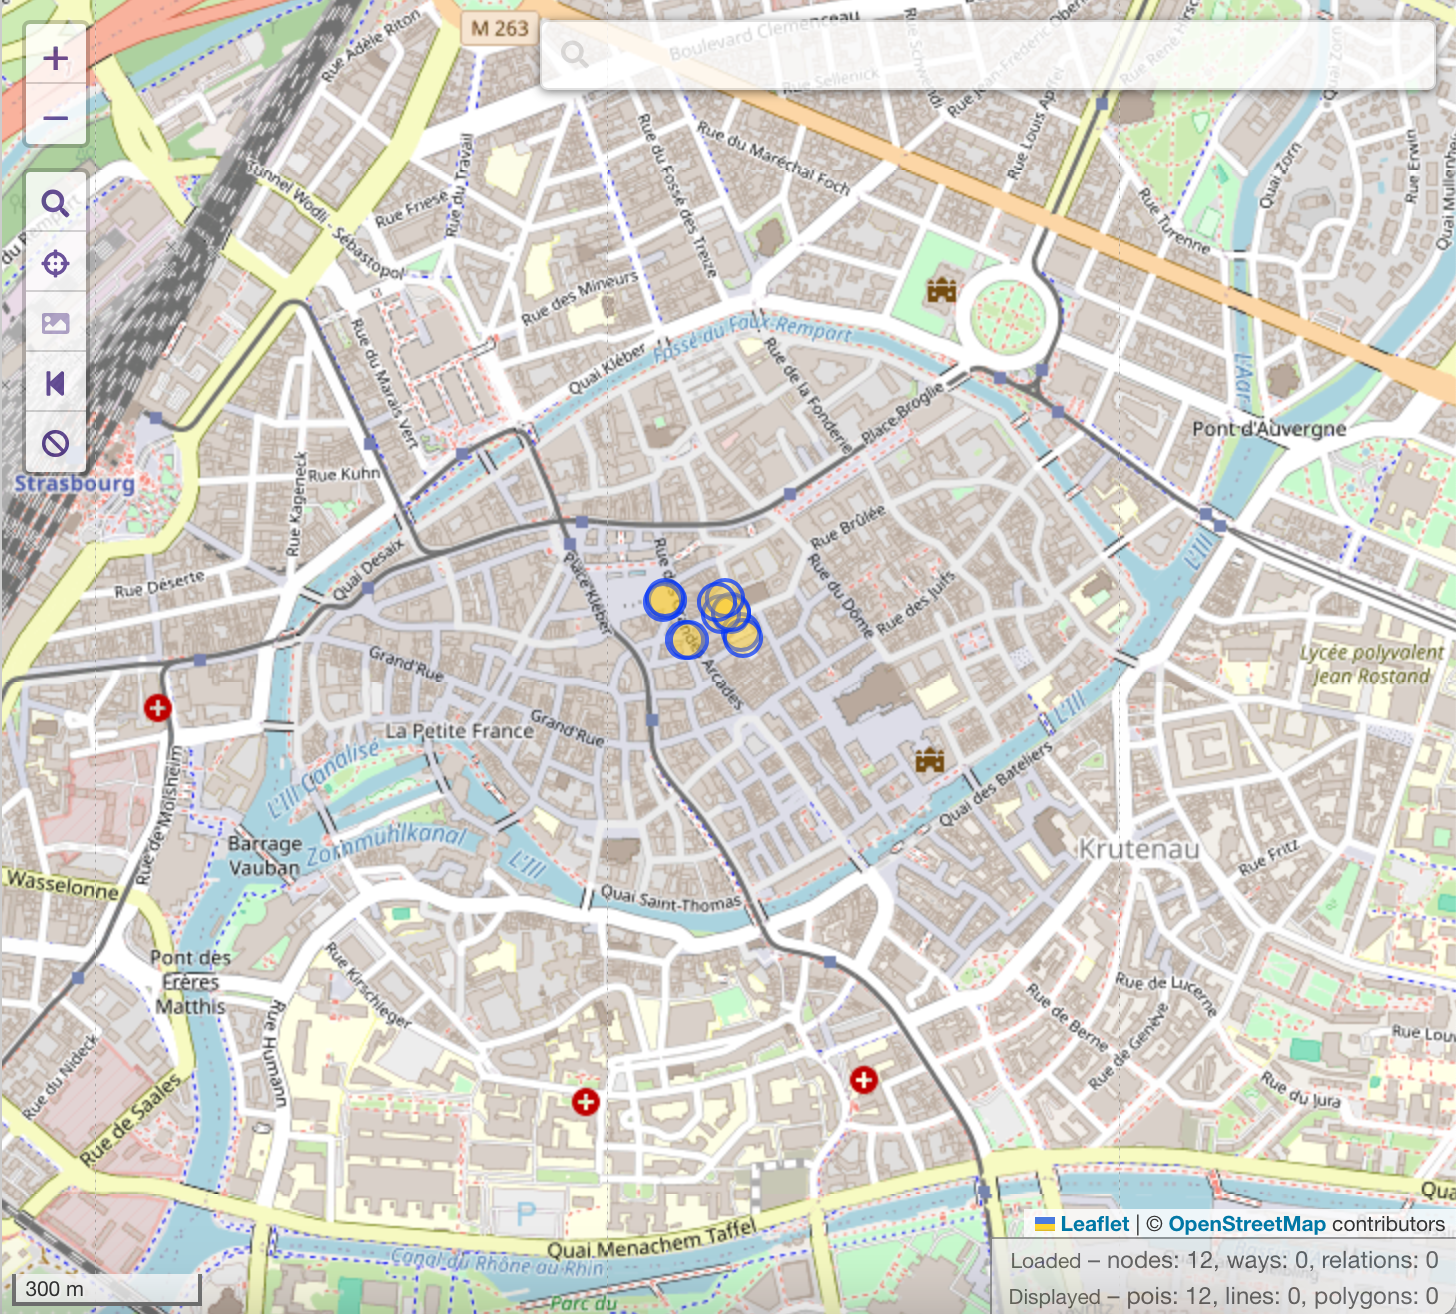
\includegraphics[width=0.7\textwidth]{images/bbox1.png}
    \captionsetup{font={scriptsize}}
    \caption{Bounding Box 1: 153.7 m², 12 trees}
\end{figure}
\end{frame}

\begin{frame}{Benchmark: bbox 2}
  \begin{figure}[H]
    \centering
    \includegraphics[width=0.7\textwidth]{images/bbox2.png}
    \captionsetup{font={scriptsize}}
    \caption{Bounding Box 2: 384.0 m², 71 trees}
\end{figure}
\end{frame}

\begin{frame}{Benchmark: bbox 3}
  \begin{figure}[H]
    \centering
    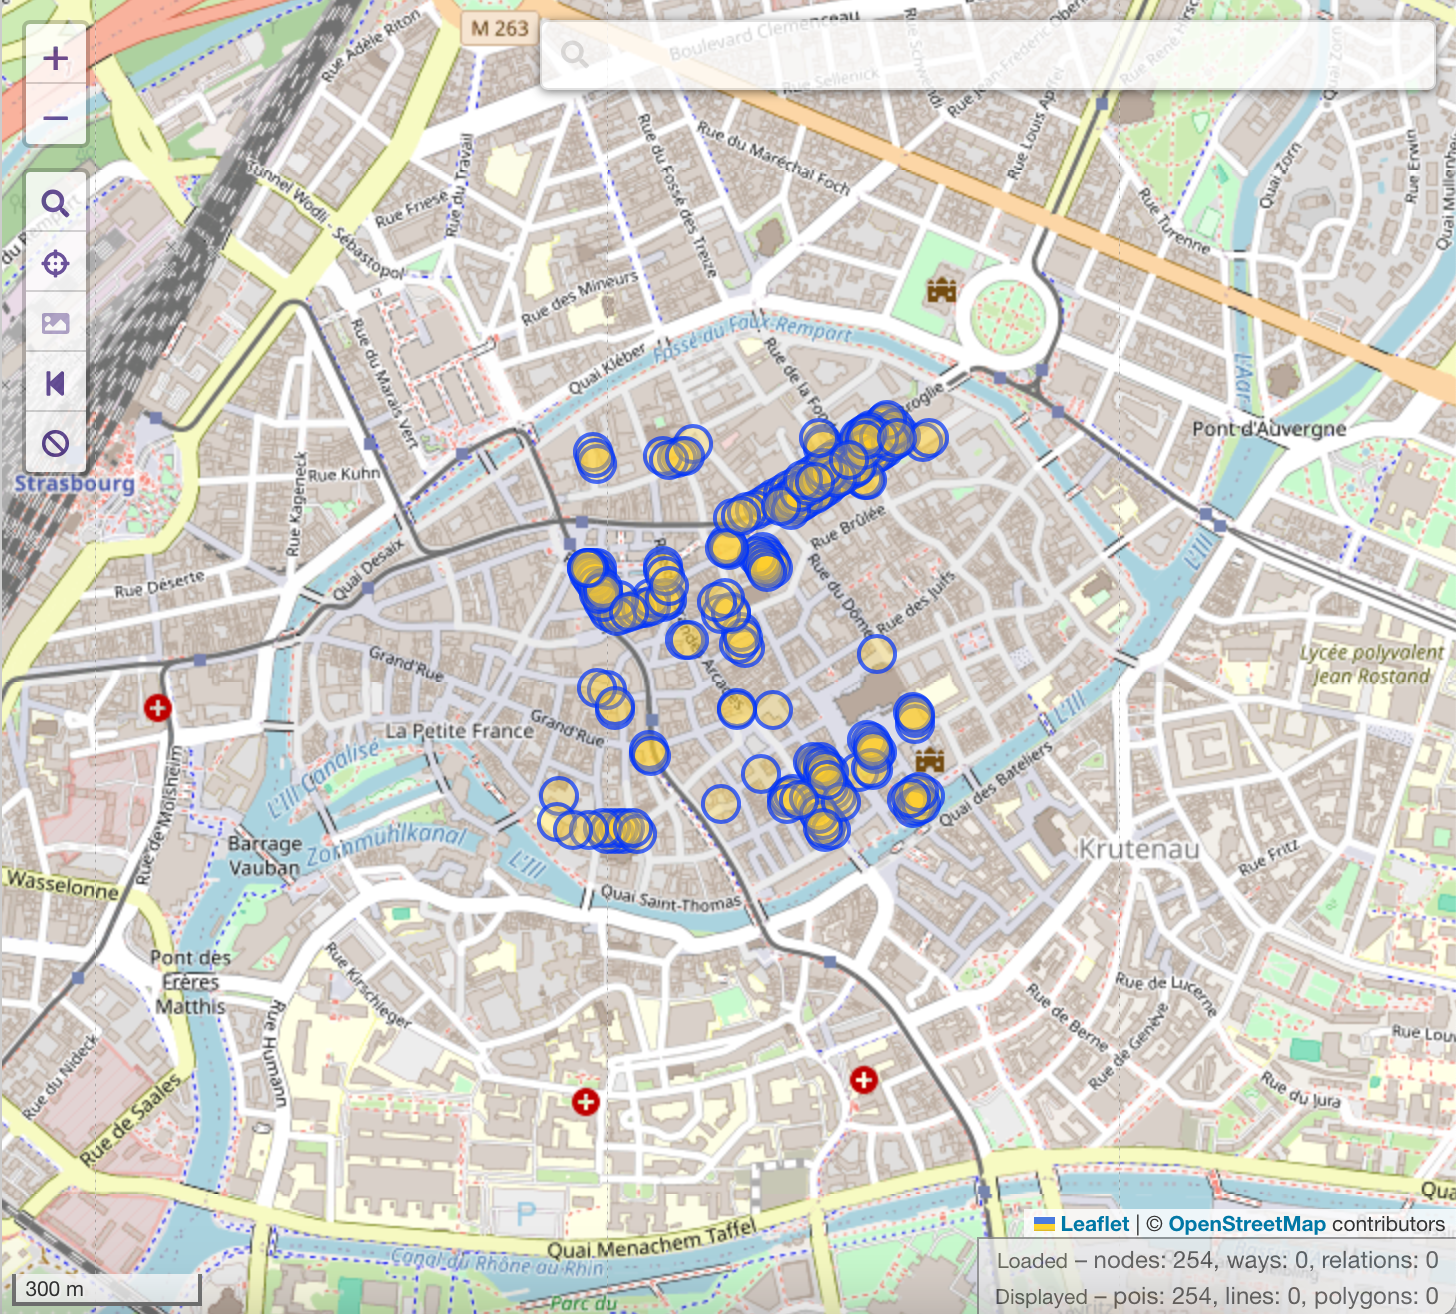
\includegraphics[width=0.7\textwidth]{images/bbox3.png}
    \captionsetup{font={scriptsize}}
    \caption{Bounding Box 3: 626.1 m², 254 trees}
\end{figure}
\end{frame}

\begin{frame}{Benchmark: bbox 4}
  \begin{figure}[H]
    \centering
    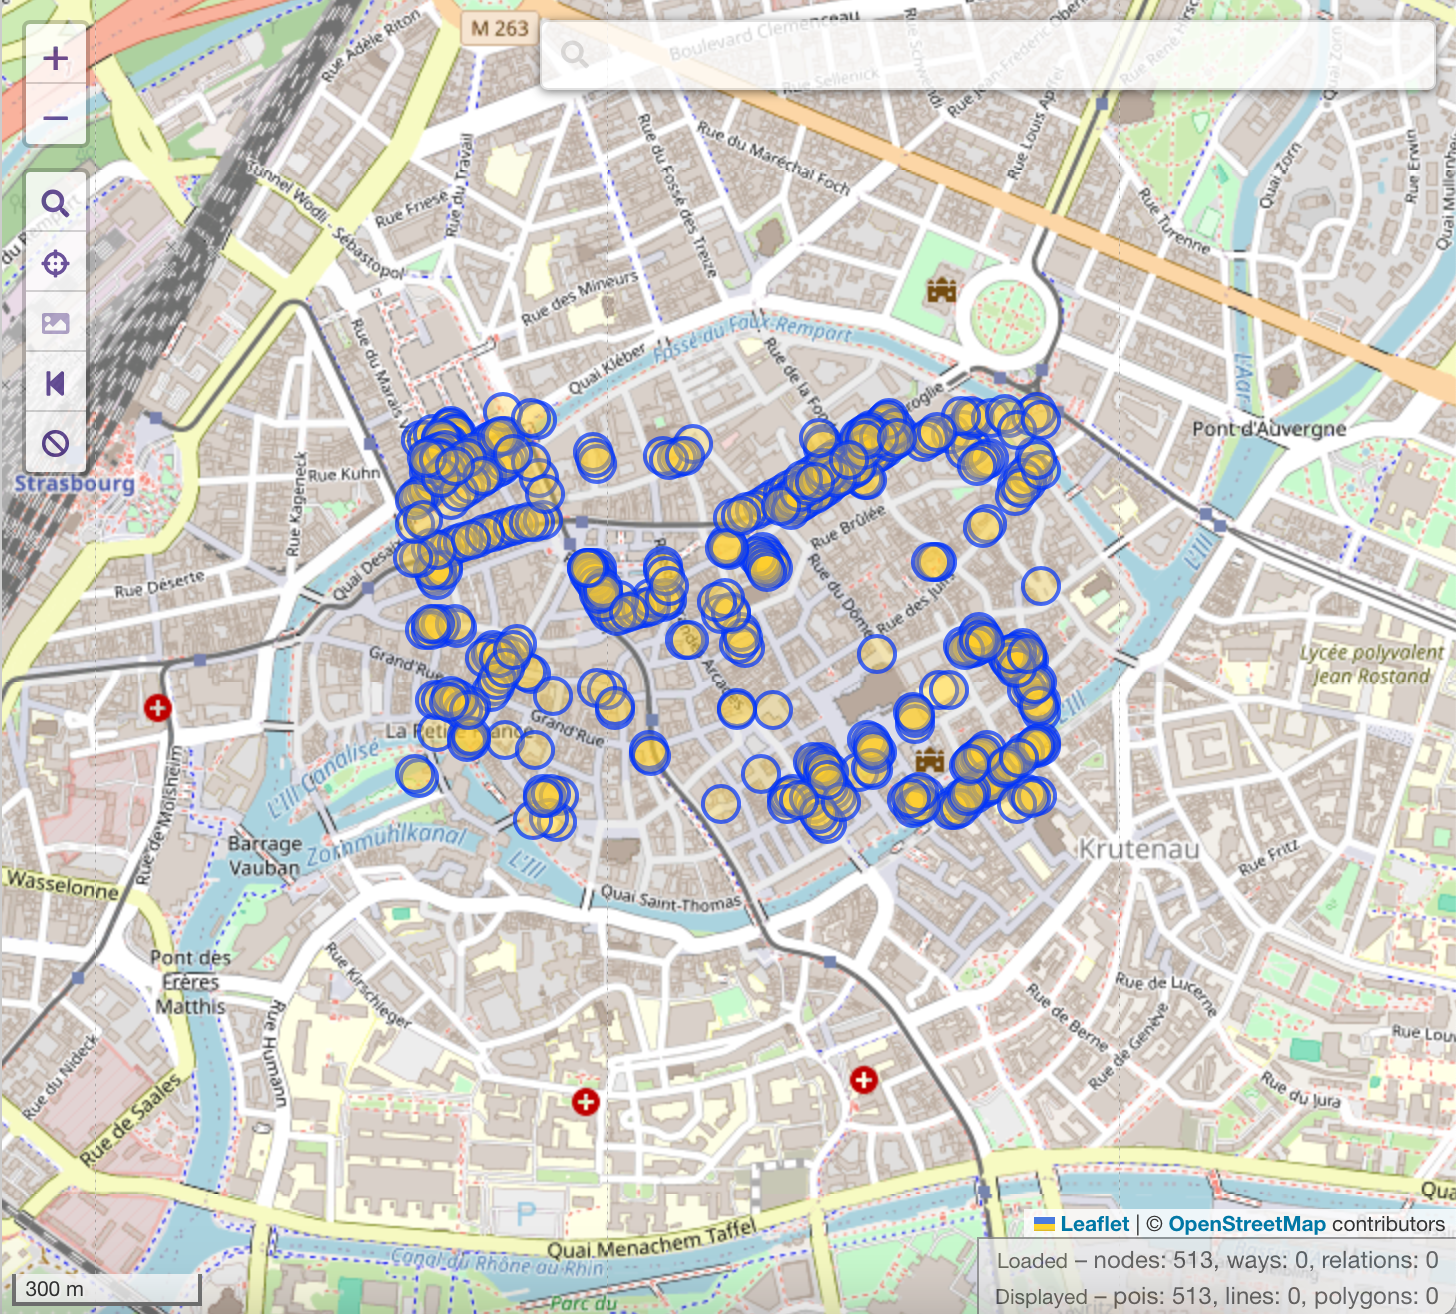
\includegraphics[width=0.7\textwidth]{images/bbox4.png}
    \captionsetup{font={scriptsize}}
    \caption{Bounding Box 4: 808.4 m², 513 trees}
\end{figure}
\end{frame}

\begin{frame}{Benchmark: relation LOD-number of faces}
  \begin{figure}[H]
    \centering
    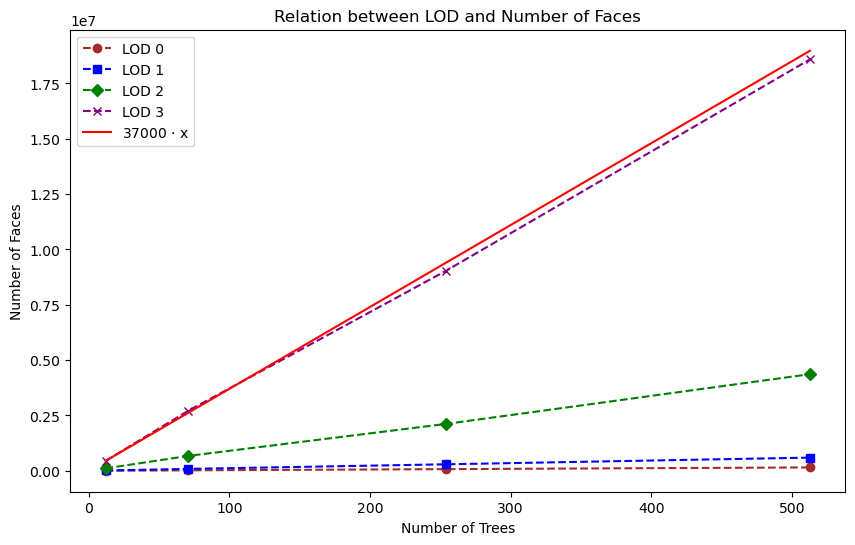
\includegraphics[width=0.8\textwidth]{images/bench_ntree_nfaces.png}
    \captionsetup{font={scriptsize}}
\end{figure}
Linear relation between the number of faces and the number of trees.
\end{frame}

\begin{frame}{Benchmark: execution time}
  \begin{figure}[H]
    \centering
    \includegraphics[width=0.8\textwidth]{images/bench_time_ntree.png}
    \captionsetup{font={scriptsize}}
\end{figure}
Quadratic relation between the number of trees and the execution time.
\end{frame}



% \nocite{*}
\bibliographystyle{plain}
\bibliography{references}

\end{document}